\documentclass{article}

\usepackage{graphicx}
\usepackage{geometry}
\usepackage{multicol}
\usepackage{gensymb}
\usepackage{mathtools}
\DeclarePairedDelimiter\bra{\langle}{\rvert}
\DeclarePairedDelimiter\ket{\lvert}{\rangle}
\DeclarePairedDelimiterX\braket[2]{\langle}{\rangle}{#1 \delimsize\vert #2}
\usepackage{amsmath}
\usepackage{titlesec}
\usepackage{lipsum}
\usepackage{setspace}


\usepackage[
backend=biber,
style=numeric,
sorting=none
]{biblatex}
\addbibresource{bibliography.bib}

 \geometry{
 a4paper,
 total={170mm,257mm},https://www.overleaf.com/project/5e3c23cf3375b0000167df84
 left=20mm,
 top=20mm,
 }
 

\setlength{\columnsep}{0.4cm}

\begin{document}



\title{Investigating applications of transient effects in the optical pumping of rubidium isotopes in simulating qubits under Rabi oscillations }
\author{u1703249, u1617871, u1705902}
\date{Department of Physics, University of Warwick, Coventry, CV4 7AL, United Kingdom}

%-----------------------------------------
\maketitle
The Larmor frequency, $\omega_0$, for a sample of $^{85}$Rb and $^{87}$Rb isotopes kept at a constant temperature of 50.0$^{\circ}$C is measured as a function of radio frequency (RF) amplitude at resonance frequencies for an optically pumped system with a periodically applied RF field. The ratio of the landau g factors for $^{85}$Rb and $^{87}$Rb isotopes is calculated by finding the ratio of the gradients of the line of best fit for the 2 isotopes. The value of the ratio is 1.48$\pm$0.05. At high fields when the RF is applied and transient effects are observed during the defined characteristic timescale $\tau_c=6\times10^{-4}$[s], the system behaves as a collection of quantum qubits driven by a Rabi oscillation before decoherence dominates. Adjusting the field to act on the system for a time $t_{\pi}=1.76\pm0.10\times10^{-4}$[s], a $\pi$ pulse, and $t_{\frac{\pi}{2}}=0.86\pm0.02\times10^{-4}$[s], a $\frac{\pi}{2}$ pulse, corresponds to the transitions $\ket{0}\longrightarrow\ket{1}$ and
$\ket{0} \longrightarrow\frac{\ket{0}+i\ket{1}}{\sqrt{2}}$ respectively.

%-----------------------------------------


\sloppy
\begin{multicols*}{2}

\setlength{\parindent}{4ex}
\setlength{\parskip}{0em}

\section{Introduction}

In optical pumping, circularly polarised photons selectively filtered from linearly polarised light $\pi$,
\begin{equation}\label{polarization}
\setlength{\abovedisplayskip}{3pt}
    \pi = \frac{1}{\sqrt{2}}[\sigma _{+} \pm \sigma_{-}]
\setlength{\belowdisplayskip}{3pt}
\end{equation}
 redistribute the electronic states of a sample of rubidium atoms. ($\sigma _{+}$ represents right-hand circularly polarised light and $\m \sigma_{-}$ represents left-hand circularly polarised light). Free rubidium atoms are modelled as a simple hydrogenic system with only the single valence electron investigated. This polarisation imposes a selection rule on the system, therefore providing a constraint on the possible electronic transitions. 

In quantum computing, a qubit, the basic unit of quantum information, is described as a coherent superposition of two quantum states, labelled $|0\rangle$ and $|1\rangle$. \cite{nielsen}. Quantum operations on qubits, i.e. quantum logic gates, form the basis of quantum circuits where initialising the system of qubits is equivalent to identifying the initial state of each qubit.

In particular, we hypothesise the selection rules defined by the polarisation of light may be used in optical pumping to quench our system to a higher energetic state, $|0\rangle$ or a lower  energetic state $|1\rangle$, therefore completely determining the initial state of the system. 

Quantum Supremacy, the hypothesis that quantum processors execute algorithms at an exponentially faster rate compared to classical processors has been supported by experimental evidence by Google \cite{arute}. Quantum algorithms offer a more than polynomial complexity advantage over the most optimal classical algorithms including simulations in solid state physics \cite{aspuru}, approximation of Jones polynomials \cite{wocjan}, and solving Pell's equation \cite{hallgren}.

It is therefore crucial that further experiments are carried out to investigate feasible regimes in which quantum logic gates can be simulated. In optical pumping we demonstrate that for a short timescale the cloud of rubidium gas can be modelled as a collection of qubits with well-posed initial conditions.


\section{Theory}

\subsection{Optical Pumping and Transient Effects}

Denoting the total angular momentum of an atom by $\textbf{F}$, applying a weak external field $\textbf{B}$ to the atom is equivalent to introducing a quantum perturbation to the Hamiltonian. The magnetic quantum number $\textbf{M}$ is defined as the component of $\textbf{F}$ in the direction of $\textbf{B}$. The perturbation due to the external field $\textbf{B}$ results in Zeeman splitting, lifting the degeneracy of the $\textbf{F}$ states, allowing for the possibility of more electronic energy transitions.


Right-hand circularly polarized light travelling in the direction of $\textbf{B}$ imposes the selection rule  $\mathrm{\triangle M = +1}$. If the direction of polarization or direction of the field is reversed, then the selection rule becomes $\mathrm{\triangle M = -1}$.

The selection rule for $\textbf{M}$ during a  transition from $\mathrm{^{2}P_{\frac{1}{2}}}$ to $\mathrm{^{2}S_{\frac{1}{2}}}$  is given by $\mathrm{\triangle M = 0, \pm 1}$, where $\mathrm{^{2}S_{\frac{1}{2}}}$ and $\mathrm{^{2}P_{\frac{1}{2}}}$ are the degenerate ground state and first excited state respectively.

The atoms are excited by incident photons, raising their energy levels provided the selection rules are obeyed. This is followed by stimulated emission, where the atoms de-excite and emit radiation isotropically. As a result, the atoms populate the $\mathrm{F = 2, M = 2}$ sublevel of the $\mathrm{^{2}S_{\frac{1}{2}}}$ state. Since there is no M = 3 sublevel in the $\mathrm{^{2}P_{\frac{1}{2}}}$ state, electrons in the $\mathrm{F=2, M=2}$ sublevel of the $\mathrm{^{2}S_{\frac{1}{2}}}$ state cannot absorb any more photons and the atom is said to be optically pumped.

To induce transitions between energy levels for each rubidium isotope, a steady radio frequency (RF) magnetic field is applied perpendicular to the external weak field. This RF field induces transitions with $\mathrm{\triangle M = \pm 1}$, driving the system back towards the ground state, allowing absorption of photons. The frequency of the RF field at which this occurs differs for each isotope of rubidium and the dips in observed light intensity are called resonances.

To study transient effects, the RF field is rapidly switched on and off by the application of a high frequency square pulse with the weak field held constant at a value $B_{0}$ at the centre of a resonance. Pumping results in an excess population in the M = 2 state while the RF field is off. 

The M = 1 and M = 2 sub-levels have populations $p_{1}$ and $p_{2}$ respectively. If $b_{12}$ is defined to be the transition probability from the state M = 1 to M = 2, and $b_{21}$ is the transition probability from state M = 2 to M = 1 we have the rate equations:

\begin{equation}\label{rate1}
    \dot{p_{2}} = -b_{21}p_{2} + b_{12}p_{1}
\end{equation}
\begin{equation}\label{rate2}
    \dot{p_{1}} = -b_{12}p_{1} + b_{21}p_{2}
\end{equation}
\cite{colegrove}. But $b_{21} = b_{12} = b$ and we have a normalization condition $p_{1} + p_{2} = 1$. Denoting $\delta$ as the initial excess population in $p_{2}$, the solutions of the rate equations are
\begin{equation}\label{sol1}
    p_{1} = \frac{1}{2}-\delta e^{-2bt}
\end{equation}
\begin{equation}\label{sol2}
    p_{2} = \frac{1}{2}+\delta e^{-2bt}
\end{equation}
Since $b_{12} = b_{21}$ and $p_{2}$ is initially greater than $p_{1}$, more atoms transition to the M = 1 state, leading to a rapid decrease in observed light intensity. Now the situation is reversed, and the excess population in M = 1 will transition to M = 2. This continues and is observed as a damped sinusoidal signal, with period corresponding to the Larmor frequency 
\begin{equation}\label{larmor}
  \omega_{0} = g_{f}\frac{\mu_{0}}{\hbar} B_{0}
\end{equation}
 $\omega_{0} $ is the precession of $\textbf{F}$  about the RF field, where $g_{f}$ is the g-Landé factor, $\mu_{0}$ is the Bohr magneton and $\hbar$ is the reduced Planck's constant.

 We expect this process to take a characteristic time to achieve a suitable population in the M=2 state. Before the RF field is applied, $p_{2} = \frac{1}{2}+\delta$. The time to reach $\frac{1}{e}$ of this value is
 \begin{equation}\label{char_time}
     t_{\frac{1}{e}} = \frac{1}{2b}
 \end{equation}
 Hence, the time period is inversely proportional to the RF field amplitude \cite{teachspin}.
 
\subsection{Quantum Computing}

A quantum bit, or qubit, is a coherent superposition of basis eigenstates labelled $|0\rangle$ and $|1\rangle$, so any state $\psi$ can be described by
\begin{equation}\label{qubit_state}
    |\psi\rangle = c_{0}|0\rangle + c_{1}|1\rangle
\end{equation}
where $c_{0}$ and $c_{1}$ are complex probability amplitudes. \cite{nielsen}.
In the presence of an oscillatory driving field (the RF field), atomic two level systems display a cyclic behaviour by absorbing photons and re-emitting them.

This is called a Rabi oscillation. To control transitions between $|0\rangle$ and $|1\rangle$, the RF field is applied for a time $t_{\pi} = \frac{\pi}{\omega_{0}}$, known as a $\pi$ pulse. Applying a $\frac{\pi}{2}$ pulse, $t_{\frac{\pi}{2}} = \frac{\pi}{2\omega_{0}}$, puts the qubit into a superposition
\begin{equation}\label{superposition}
|0\rangle \longrightarrow \frac{|0\rangle+i|1\rangle}{\sqrt{2}}
\end{equation}
\cite{bellac}. The operation that switches between eigenstates introduces a random phase $\phi$, given by a Gaussian distribution
\begin{equation}\label{phase_gauss}
    p(\phi) = (4\pi\alpha)^{-\frac{1}{2}}e^{\frac{-\phi^{2}}{4\alpha}}
\end{equation}
where $\alpha$ is the variance of the phases, so the eigenstates transform as 
\begin{equation}\label{state_transform_1}
    |0\rangle \longrightarrow |0\rangle 
\end{equation}
\begin{equation}\label{state_transform_2}
    |1\rangle \longrightarrow e^{i\phi}|1\rangle 
\end{equation}


Therefore, after several flips, measurements cannot distinguish between the eigenstates, showing decoherence. This can be seen in the density matrix for a general state $\psi_{j}$,
\begin{equation}\label{density_mat}
    \rho_{j} = \begin{pmatrix}
    |c_{0}|^{2} & c_{0}c_{1}^{*}e^{-\alpha}\\
    c_{0}^{*}c_{1}e^{-\alpha} & |c_{1}|^{2}
    \end{pmatrix}
\end{equation}
where the off-diagonal terms decay with increasing $\alpha$. The time taken for the off-diagonal terms to effectively vanish is called the decoherence time \cite{zurek}, and this can be identified with $t_{\frac{1}{e}}$.

Consequently, any pulses applied to control the qubit states must be applied before decoherence. 


\section{Methodology}

An RF lamp containing $^{85}$Rb, $^{87}$Rb, and xenon gas is heated to produce a beam of resonance light through excitation of the rubidium atoms. The light from the lamp consists of two main lines: one at 780nm and one at 795nm. The beam is collimated by a plano-convex focusing lens and is made monochromatic by passing through an interference filter that isolates the light corresponding to the 795nm line. The beam then passes through a linear polarizer and a quarter wave plate making it circularly polarized. This light passes through the oven which contains a $^{85}$Rb and $^{87}$Rb vapour absorption cell. After leaving the oven, the diverging light is focused onto the photodiode by a second plano-convex lens.
%\begin{center}
\begin{Figure}
\centering
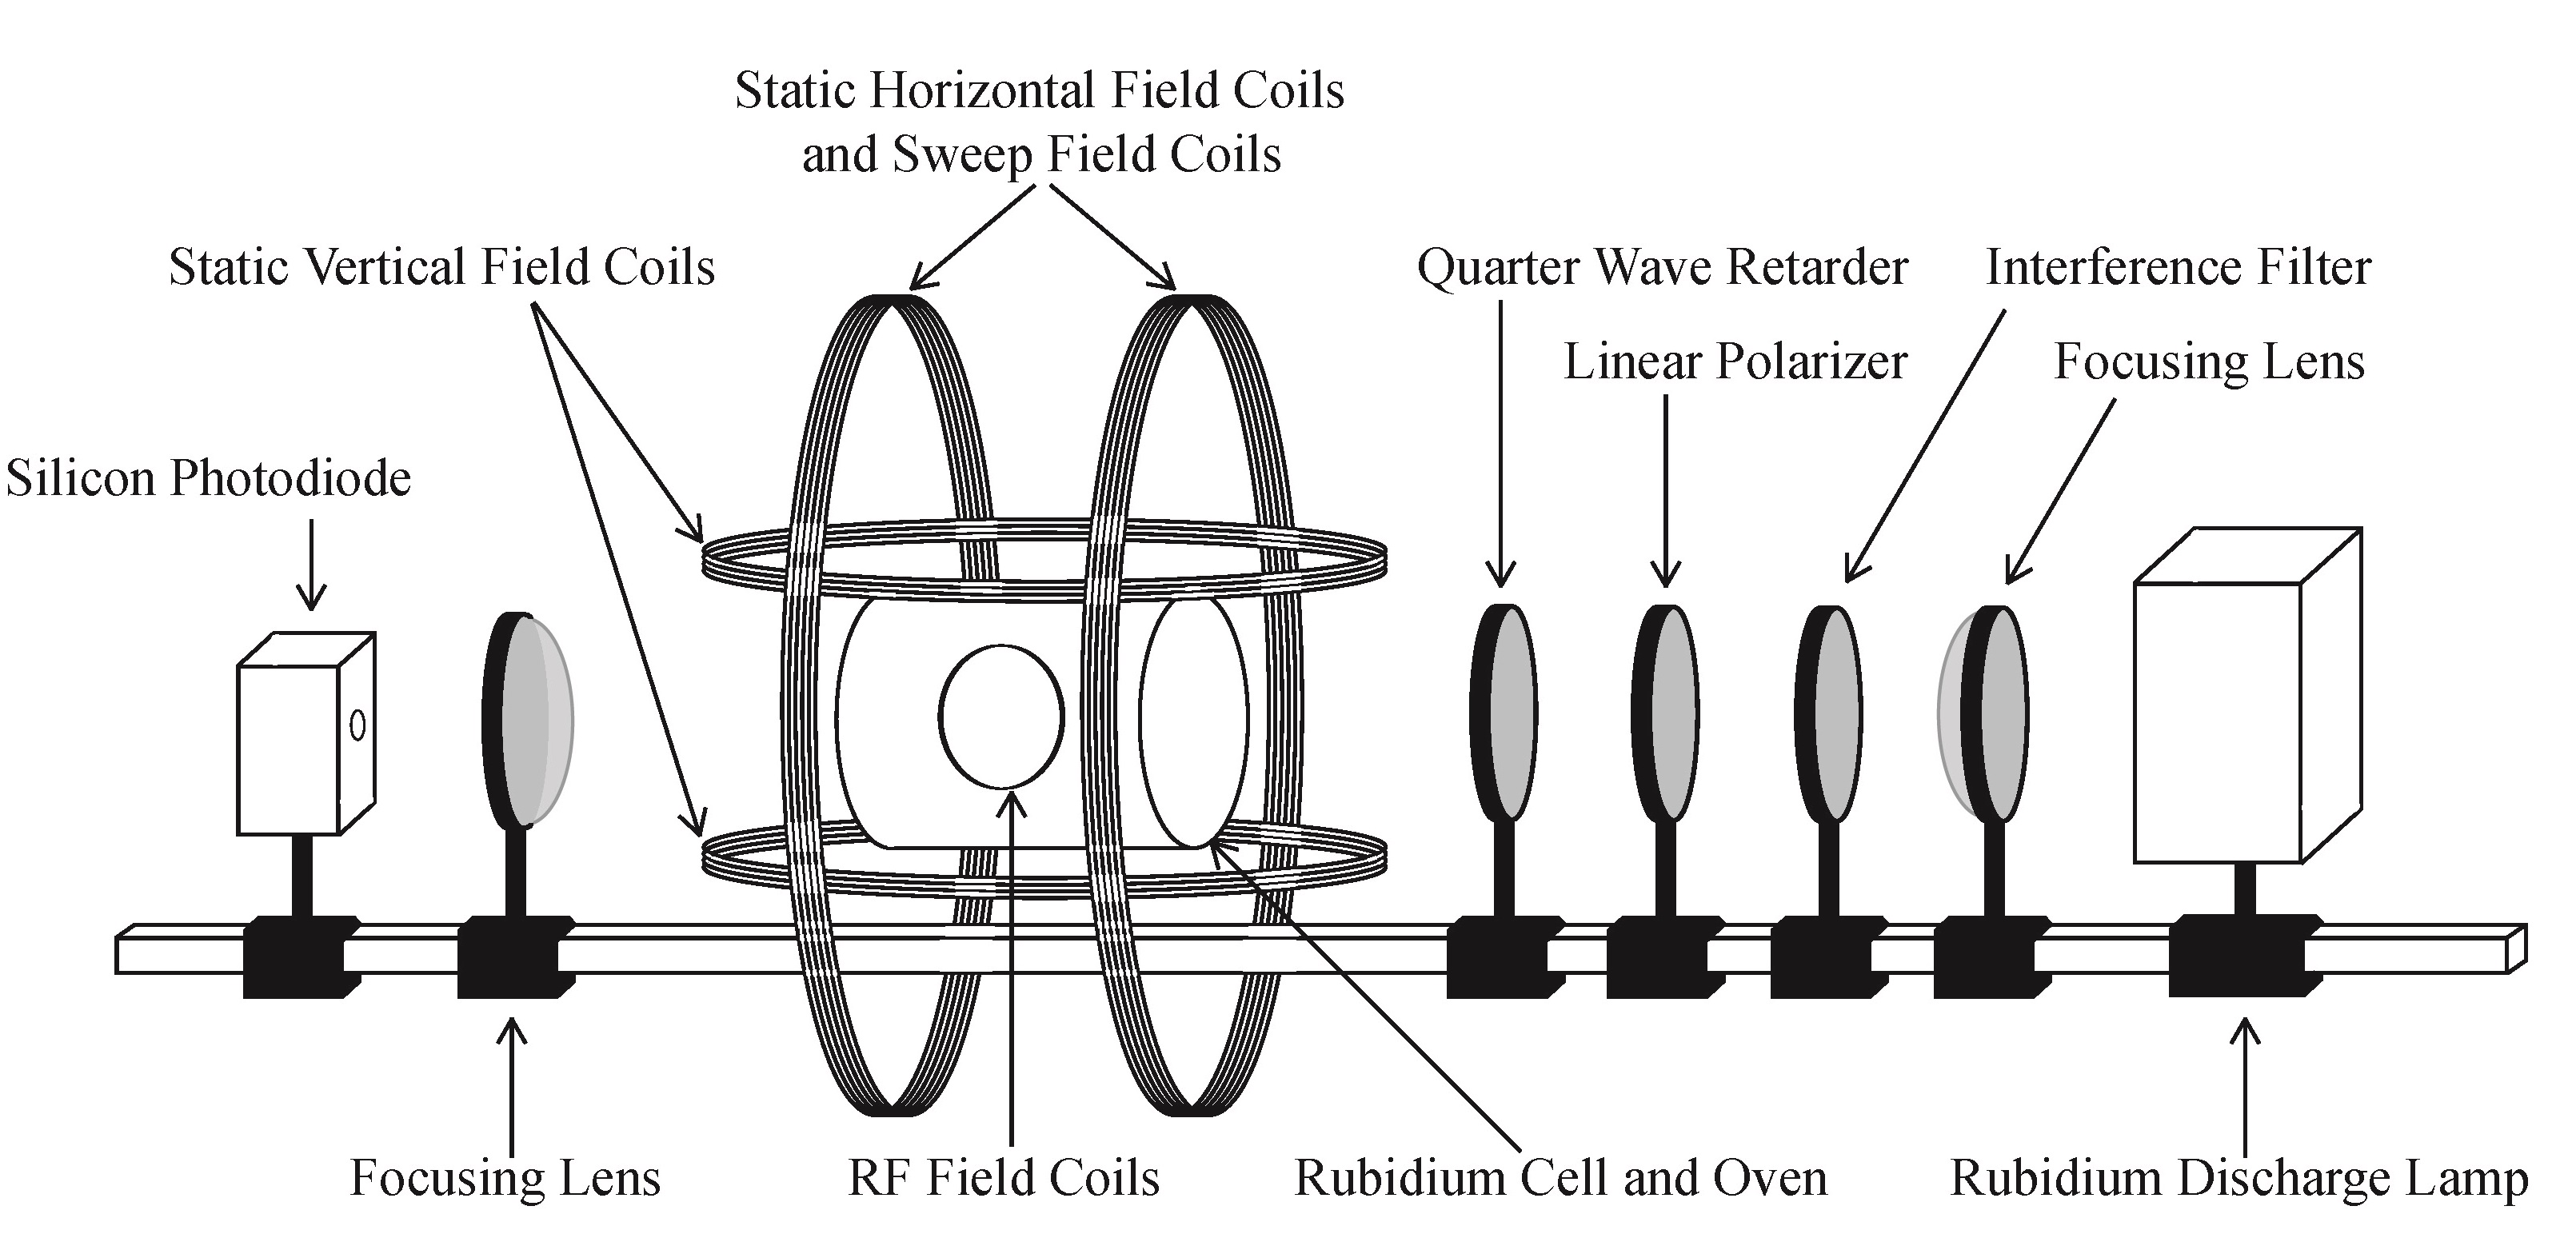
\includegraphics[width=\linewidth]{apparatus.jpg}
\footnotesize
Figure 1. The apparatus used in the experiment. \cite{apparatus}.
\normalsize
\vspace{5mm} %5mm vertical space
%\end{center}
\end{Figure}

The current through the vertical and horizontal coils (the primary coils) is set such that they produce a static field either parallel or anti-parallel to the Earth's local magnetic field. Inhomogeneity in the third component of the Earth's field is minimised by aligning the apparatus so that its main axis is parallel to the local field. The currents in the primary coils is kept constant and the orientation of the apparatus is not changed throughout the experiment so that the Earth's field is interfered with consistently. The apparatus for the experiment is shown in Figure 1.

A square wave pulse of amplitude 0 to +5.0V with frequency 4.98Hz is connected to the RF modulation input using a signal generator. The voltage of the photodiode is shown by an oscilloscope connected to it, which is set to trigger at the falling edge of the square wave. The sinusoidal decay and exponential rise of the light intensity is extracted from the oscilloscope for a range of different values of RF field amplitudes. This is done at the resonances of each rubidium isotope.

The temperature of the lamp is held constant at 50.0$^{\circ}$C to keep the intensity of the resonance light constant and the frequency of the RF field is held constant at 139.6kHz in order to isolate the effect of the RF field amplitude only.

\section{Results}
When the RF is applied periodically, quantum theory predicts the transmitted light intensity will rapidly decrease and then increase as the atoms transition between the M=2 and M=1 states. Results have been plotted with a vertical scale of $5\times10^{-1}$ [V] and a horizontal scale of 2.5$\times10^{-4}$ [s]. When light intensity is plotted against time we expect it to take the shape of a damped signal. This can be seen on Figure 2, with the frequency corresponding to $\omega_{0}$. 
\newline

\begin{Figure}
\begin{center}
\includegraphics[width=\linewidth]{Graph15.jpg}
\end{center}
\footnotesize
    Figure 2. The region during which the RF turns on and the damped signal can be observed as the system transitions between the pumped and non-pumped states.
\normalsize
\vspace{0.2mm}
\end{Figure}
\newline

We investigate the relationship between the RF amplitude in units of [V] and the period of oscillation $\omega _{0^{-1}}$ in units of [s]. Equation (\ref{larmor}) suggests that there is a linear relationship between the inverse RF amplitude and the oscillation period. The straight line correlation can be observed on Figure 3 for both $^{87}\mathrm{Rb}$
and $^{85}\mathrm{Rb}$ respectively. For $^{87}\mathrm{Rb}$ the data points are grouped closer to the line of best fit when directly compared with $^{85}\mathrm{Rb}$. This could be due to noise from the 50Hz mains supply altering our measurements. The gradient of the line of best fit are given by 441.7$\pm$2.7 and 298.8$\pm$8.3 for $^{87}\mathrm{Rb}$ and $^{85}\mathrm{Rb}$  respectively. The experimental value of the ratio of the Landau $g$ factors $g_f$ can be obtained from dividing the gradients of the lines of best fit. For $^{85}\mathrm{Rb}$ and $^{87}\mathrm{Rb}$ this ratio is given by 1.48$\pm$0.05. Comparison with the theoretical value of 1.50, our results confirm the theory given that it lies within the uncertainty bounds. Confirming this theoretical value suggests predictions of our experimental setup agree with theoretical values and therefore allows us to further investigate transient effects.
\\

\newline
\begin{Figure}
%\begin{center}
\centering
\includegraphics[width=\linewidth]{transient.jpg}
%\end{center}

\footnotesize
    Figure 3. Linear correlation between the inverse RF amplitude [V$^{-1}$] and time [s]. Error bars are present however they can not be seen as they are insignificant compared to the scale of the system. The corresponding gradients for the line of best fit are 441.7$\pm$2.7 and 298.8$\pm$8.3 for $^{87}\mathrm{Rb}$ and $^{85}\mathrm{Rb}$ respectively. The ratio of the landau g factors are given by the ratio of the gradients. This ratio is given by  1.48$\pm$0.05.
\normalsize
\end{Figure}
\newline

When the RF field is turned on, for a short period of time the system behaves as an ensemble of qubits, transitioning from $\ket{0}$ to $\ket{1}$, driven by a perfect Rabi oscillator, and taking the population of the system from the M=2 state to a non pumped state. $\ket{0}$ represents the initial pumped state at t=0 [s]. The data has been extracted from an oscilloscope at higher fields with an RF frequency of 4.00MHz with a corresponding RF amplitude of 5.2 [V]. The period for the Rabi oscillation is given by T$_r$=$1.72\pm0.03\times10^{-5}$ [s]. Decoherence becomes dominant the longer we leave the RF field running. This can be observed as the system is transitioning from the initial $\ket{0}$ to the $\frac{\ket{0}+i\ket{1}}{\sqrt{2}}$ state, redistributing itself according to equations (\ref{sol1}) and (\ref{sol2}). 

We define the characteristic timescale as $\tau_c=6\times10^{-4}$s where the system is behaving as a quantum qubit driven by a perfect Rabi oscillation. In our characteristic timescale $\tau_c$, a $\pi$ pulse can be achieved by turning on the RF for $t_{\pi}=1.76\pm0.10\times10^{-4}$ [s] which corresponds to the $\ket{0}\longrightarrow\ket{1}$ transition. A $\frac{\pi}{2}$ pulse is achieved at a time $t_{\frac{\pi}{2}}=0.86\pm0.02\times10^{-4}$ [s] which corresponds to the mixed state defined by (\ref{superposition}). In our experiment, decoherence occurs due to external factors. Examples include uncertainty in the exact wavelength $\lambda$ of the laser and the frequency of our RF field as well as phonon interactions and disturbances caused by the fields generated by each individual atom.These external factors contribute to our random phase defined by (\ref{state_transform_2}) where the phase distribution due to the uncertainties cause the Rabi frequency to turn into a distribution $\omega \longrightarrow \int f(\omega)d\omega$.
\\

\begin{Figure}
%\begin{center}
\centering
\includegraphics[width=\linewidth]{rabi_oscill_close.jpg}
\footnotesize
    Figure 4. Rabi oscillations are observed with a period of T$_r$=$1.72\pm0.03\times10^{-5}$ [s] at a temperature T=50.0$^\circ$C when the RF field is turned on. The period has been obtained from a sinusoidal wave fit (red) for the duration of the characteristic time scale $\tau_c$ before quantum decoherence becomes dominant. The $\pi$ and $\frac{\pi}{2}$ pulses are achieved at $t_{\pi}=1.76\pm0.10\times10^{-4}$ [s] and $t_{\frac{\pi}{2}}=0.86\pm0.02\times10^{-4}$ [s] respectively.
\normalsize
%\end{center}
\end{Figure}
\newline
\begin{Figure}
%\begin{center}
\centering
\includegraphics[width=\linewidth]{rabi_oscil.jpg}
\footnotesize
    \setstretch{0.5}
    Figure 5. Observed light intensity against time [s] for high field Rabi oscillations.
\normalsize
%\end{center}
\end{Figure}
\\
\newline
 Outside our defined characteristic timescale $\tau_c$, the $\alpha$ factor in (\ref{density_mat}) increases as decoherence becomes more dominant. The states become indistinguishable as they are transitioning to the new equilibrium state, meaning quantum information is lost about the system and the qubit is destroyed. This is observed on Figure 5 where the light intensity starts to converge to a steady value.


\section{Discussion}
With regards to applications to quantum logic gates, we note that it may be possible to simulate the optical pumping apparatus as a quantum Hadamard gate within the characteristic time during which Rabi oscillations are present. By altering the polarisation of photons we may quench the initial system of the system to a state of $|0\rangle$ 'qubits' or $|1\rangle$ 'qubits'. The population reversal equations predict the system will then redistribute to an equal split between  $|0\rangle$ and $|1\rangle$ states, which we may model as follows:

\begin{equation}\label{mixed_plus}
  |1\rangle \longrightarrow \frac{1}{\sqrt{2}}|0\rangle + \frac{1}{\sqrt{2}}|1\rangle  
\end{equation}

\begin{equation}\label{mixed_minus}
    |0\rangle \longrightarrow \frac{1}{\sqrt{2}}|0\rangle - \frac{1}{\sqrt{2}}|1\rangle
\end{equation}
or more concisely written as the operator $H$, where
\begin{equation}\label{h_operator}
    H = \frac{1}{\sqrt{2}}\begin{pmatrix}
1 & 1\\ 
1 & -1
\end{pmatrix}
\end{equation}
This operator defines a quantum Hadamard gate. Reversing the polarization of light also changes the selection rules for allowed transitions and the initial and final states of the system implying that when polarization is reversed the new $\ket{1}$ and $\ket{0}$ might be different from the initial $\ket{0}$ and $\ket{1}$ qubits that were used when using right hand polarized light. Furthermore, careful consideration of decoherence factors and effects must be considered and further experimentation must be conducted to verify the validity of this hypothesis and its possible applications and limitations. Decoherence presents a significant drawback, since the loss of information implies qubits become untangled. 

Recent advancements in research have shown that the NV (Nitrogen-vacancy) center in diamond, one of the numerous point defects in the material remains coherent even for extended periods of time at room temperature. These properties can be feasibly measured and initialised. Another material of interest is SiC which has a di-vacancy center, sharing similar properties to the NV center in diamond \cite{eckstein}. It would be interesting to see if an ensemble of SiC can be maintained at coherence longer than rubidium via optical pumping.

Note the mains power supply interferes with the Larmor frequency resulting in a systematic error in our results. This could be avoided applying a Fourier transform to the data and isolating the Larmor frequency.
    
\printbibliography

\end{multicols*}
\end{document}
